\chapter{Czujnik wilgotności DHT-22}
\section*{Opis}
DHT-22 jest cyfrowym oraz fabrycznie skalibrowanym czujnikiem względnej wilgotności i temperatury. Zostawł stworzony w oparciu o 8 bitowy mikrokontroler, do którego podłączone są sensory. Małe rozmiary, stabliność pomiarowa, możliwość zainstalowania czujnika na duże odległości oraz niewielki pobór energii czyni go bardzo dobrym rozwiązaniem, nawet w ciężkim warunkach.

Czujnik posiada swój własny sposób uzyskiwania pomiarów. Jest on podobny do opisanej wcześniej magistrali 1wire. Do prawidłowego działania urządzenia potrzebne jest zasilanie, linia danych, poprzez która następuje komunikacja oraz uziemienie. Należy również podłączyć do linii danych oraz zasilania rezystor podciągający o oporze około 3,3 k$\Omega$.
\section*{Dane charakterystyczne}
Jak podaje specyfikacja czujnika, może być on zasilany napięciem od 3,3 do 6 V, posiada zdolności pomiarowe: wilgotność w zakresie 0 do 100 \% (z dokładnością +-2\%) oraz temperatury od -40 do 80 stopni Celsjusza (+-0,5 stopnia).

Wygląd czujnika został przedstawiony na poniższym zdjęciu:
\begin{figure}[h]
\centering
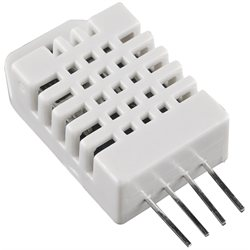
\includegraphics[scale=0.75]{dht22}
\caption{Czujnik wilgotności DHT-22}
\label{fig:dht22}
\end{figure}
\section*{Pobieranie danych z czujnika}
Zgodnie ze specyfikacją, załączoną do DHT-22, linia danych jest wolna, jeżeli jest na niej ustawiony stan wysoki. Czujnik, gdy nie jest używany, jest ustawiony w tryb spoczynku i niskiego poboru prądu. Poprzez wysłanie sygnału startu jest on wybudzany do trybu pracy i wysyła dane. Aby rozpocząć pomiar trzeba wysłać sygnał startu, należy to uczynić poprzez zwarcie do masy linii danych na conajmniej 18 ms. Po tym czasie czujnik zgłasza swoją obecność w układzie poprzez wystawienie logicznej jedynki na około 20-40 $\mu$s, następnie linia danych jest zwalniana oraz ponownie podciągana do zasilania, każdy z tych czynności trwa 80 $\mu$s. Poniższy rysunek przedstawia inicjalizację czujnika DHT-22.
\begin{figure}[h]
\centering
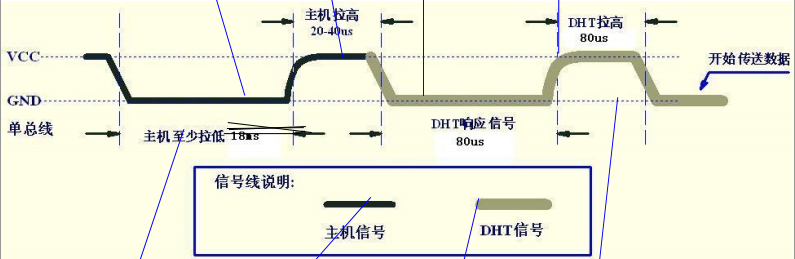
\includegraphics[scale=0.35]{inicjalizacja_dht}
\caption{Inicjalizacja czujnika}
\label{fig:inicjalizacja_dht}
\end{figure}
Po zgłoszeniu swojej obecności w układzie, czujnik zaczyna wysyłać 40 bitów danych, pierwsze 16 bitów odpowiada za ciśnienie, następne 16 to temperatura oraz końcowe 8 bitów służy jako suma kontrolna.

Aby przekonwertować odebrane dane na wskazania czujnika, należy obie liczby 16-bitowe, odpowiadające wilgotności oraz temperaturze, podzielić przez 10. W ten sposób otrzymujemy pomiary z dokładnością do jednego miejsca po przecinku. Po odebraniu danych należy przede wszystkim sprawdzić, czy to co zostało otrzymane jest prawidłowe. Należy pierwsze 4 bajty dodać do siebie oraz sprawdzić, czy 8 młodszych bitów tej wartości są równe z ostatnim odebranym bajtem. Jeżeli tak, procedura odebrania została zakończona sukcesem. W przeciwnym wypadku należy spróbować ponownie pobrać dane z czujnika.

Sposób kodowania informacji na linii danych przez DHT-22 jest następujący: każda wartość logiczna (0 oraz 1) jest reprezentowana przez podpięcie linii do zasilania na ustaloną chwilę czasową. Bit o wartości 0 jest wysyłany jako wysoki poziom przez czas 26-28 $\mu$s, natomiast czas trwania dla bitu 1 wynosci 70 $\mu$s. Pomiędzy nadaniem odpowiedniego bitu, występuje przerwa - podłączenie linii danych do uziemienia na około 50 $\mu$s.

Przebiegi poniżej pokazują wysyłanie danych:
\begin{figure}[h]
\centering
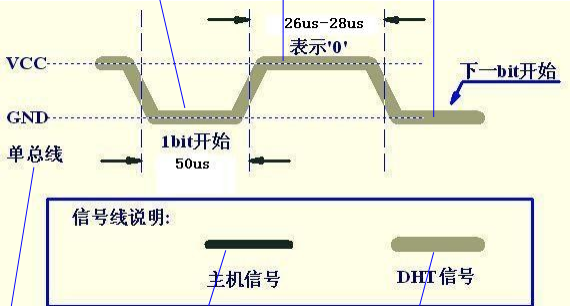
\includegraphics[scale=0.3]{zero_dht}
\caption{Wysłanie logicznego $"0"$}
\label{fig:zero_dht}
\end{figure}

\begin{figure}[h]
\centering
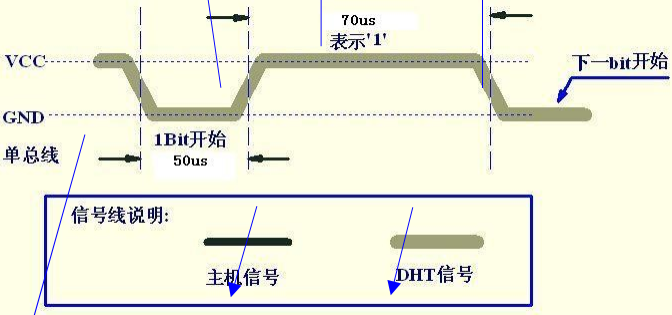
\includegraphics[scale=0.3]{jedynka_dht}
\caption{Wysłanie logicznej $"1"$}
\label{fig:jedynka_dht}
\end{figure}

Wysyłanie danych jest zakończone, jeżeli linia danych jest podłączona do zasilania oraz nie zmienia się jej stan. Czujnik wtedy przechodzi w stan uśpienia i będzie w nim przebywał aż do pojawienia się następnego sygnału startu. Jeżeli sygnał na linii danych jest zawsze w stanie wysokim, oznacza to niepoprawne działanie czujnika, może to być spowodowane wadliwym podłączeniem. 

\section*{Algorytm odczytu pomiarów}
Podczas odczytywania danych bardzo ważne są czasy występowania odpowiednich wartości logicznych. Błędna analiza czasu skutkuje złym zinterpretowaniem danych, co prowadzi do sfałszowania wyników.

Algorytm zastosowany przy tworzeniu projektu inżynierskiego jest bardzo prosty. Polega on na odczytywaniu przy każdej możliwości stanu linii danych oraz zliczaniu ilości wystąpień stanu wysokiego, gdyż tylko ten koduje wysyłane wartości z czujnika.

Linia danych jest próbkowana do momentu odczytania 40 bitów. Jest ona ustawiana wówczas w stan wysoki, czujnik przechodzi w stan spoczynku. Po zakończeniu odczytu następuje analiza przetworzonych danych.

Ilości wystąpień każdego stanu wysokiego podlegają binaryzacji, czyli procesowi podziału na dwa zbiory. Zadaniem tej funkcjonalności jest znalezienie odpowiedniej wartości granicznej, takiej która jednoznacznie wyznacza ile razy musiał być spróbkowany sygnał na linii danych, aby został on zinterpretowany jako bit $"1"$ lub $"0"$. Zostało to zaimplementowane poprzez znalezienie minimalnej i maksymalnej wartości ilości wystąpień oraz wyliczniu średniej tych dwóch liczb, wynik tego działania był wartością progową przy binaryzacji.

Po wyliczeniu progu binaryzacji, ilości wystąpień zostały poddane porównaniu z nią. Jeżeli ilość wystąpień była większa od progu, oznaczało to bit "1", w przeciwnym wypadku, było to kodowane jako "0".
\begin{figure}[h]
\centering
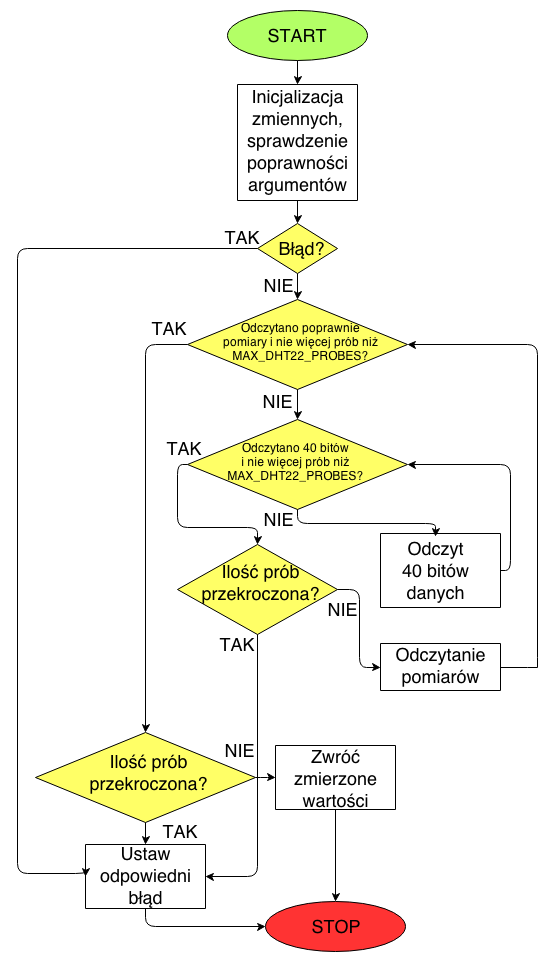
\includegraphics[scale=0.6]{diagram_dht22}
\caption{Diagram odczytu danych z czujnika DHT-22}
\label{fig:diagram_dht22}
\end{figure}